\chapter{Kapitel III - NoSQL - Ausgewählte Systeme Unboxed}
\section{ArangoDB}
ArangoDB ist gehört zu den \ac{NoSQL} Datenbanken. Die Datenbank ist besonders bekannt für ihr Multi-Modell. Multi-Modell bedeutet, dass ein \ac{DBS} mehrere Datenmodelle besitzt. Welche diese sind und wie ArangoDB funktioniert und aufgebaut ist, wird in diesem Kapitel erörtert.
\subsection{Anwendungsumfeld}
In vielen Softwareprojekten steht am Anfang nicht fest welches \ac{DBS} das beste für sie sei. Jede Datenbank bringt seine eigenen Vorteile und Nachteile mit sich. Und genau an dieser Stelle spielt ArangoDB eine wichtige Rolle:
Durch sein ’natives’ Multi-Modell ermöglicht es die Vor- und Nachteile von Datenbankmodellen auszugleichen. Dadurch wird ArangoDB zur ’Multi-Purpose-Datenbank’ mit einem dokumentenbasierten Basismodell\cite{jaxenter01}. Es kann bei einer agilen Vorgehensweise mit stetig wechselnden Anforderungen sehr Vorteilhaft sein, ein ebenso flexibles DBS wie ArangoDB zu verwenden.

 \subsection{Technologische Aspekte}
Der Kern der ArangoDB ist sein vielseitiges Multi-Modell, welches insgesamt aus drei verschiedenen Datenbank-Modellen besteht. Diese sind zu einem Modell vereint und können je nach Anwendungsfall eingesetzt werden. Das Multi-Modell besteht aus folgenden  vereinten Datenbankmodellen:

\paragraph{Das dokumentbasierte Modell} dient als solide Basis für das \ac{DBS}. Im Modell wird \ac{JSON} als Speicherformat verwendet. Durch seine Semi-Struktur und hirarschichen Aufbau ist  ein dokumentenbasiertes Modell für viele Anwendungsfälle geeignet\cite{AWS_doc}.  Außerdem bietet es eine gute Grundlage für die beiden anderen Datenmodelle.

\paragraph{Das graphbasiertes Modell} bietet die Möglichkeit Beziehungen zwischen Objekten im dokumentenbasierten Modell abzubilden. Außerdem hilft das graphbasierte Modell Datenstrukturen leichter zu verstehen und JOINs schneller aufzulösen \cite{AWS_graph}. Des Weiteren können sogennante Super-Nodes identifiziert und anschließen optimiert werden, damit der Zugriff auf diese Objekte performanter ist.

\paragraph{Das Key-Value-Modell} ist dafür optimiert Objekte zu einen gewissen Schlüssel schell abzurufen.  Anstatt lange Querys schreiben zu müssen, hilft das Key-Value-Modell optimiert auf diese Werte zuzugreifen. Optimal partitionierte Datensätze durch den geschaffenen Index sind dabei ein großer Vorteil. \cite{AWS_keyvalue}

Zusammenfassend kann man sagen, dass ArangoDB durch die Kombination der drei Datenbankmodellen ein perfektes Modell für fast jeden Anwendungsfall vorweist. Allerdings hat die Vereinigung der Modelle auch Nachteile. ArangoDB bietet zwar dem Nutzer das passende Modell für seinen Anwendungsfall, hat jedoch keine Chance gegenüber der Performance von Datenbanken, die diese Modelle nativ implementieren \cite{ADB_benchmark}.

\subsubsection{Systemarchitektur}
ArangoDB erfüllt im Clusterbetrieb das "CP" des CAP-Theorems \cite{CAP}. Mit seinem Prinzip des 'Master/Master'-Ansatzes ermöglicht es eine hohe Partitionsmöglichkeit und liefert immer die aktuellsten Daten zurück. Ermöglicht wird dies durch die Bereitstellung der drei verschiedenen Komponenten im Clusterbetrieb \cite{ADB_clusterarch}:
\paragraph{Agenten} 
beinhalten die Konfiguration des Clusters. Agenten wissen wie viele DB-Server im Cluster verfügbar sind, wo sich diese befinden und welche Daten diese enthalten. Außerdem kümmern sie sich im synchronität der verschiedenen Datenbankinstanzen im Cluster. Demnach führen diese Komponenten auch Transaktionen auf dem Datenbankcluster aus. Von dem ArangoDB-Team werden Agenten auch als Herz des Clusters bezeichnet. \cite{ADB_clusterarch}
\paragraph{Koordinatoren} bilden die Schnittstelle zum Cluster. Sie kümmern sich um Abfragen mit \ac{AQL} an die Datenbanken oder implementieren Foxx Microservices in ihrer Architektur. Die Koordinatoren wissen, welcher der optimalste Weg für die Datenabfrage ist und sammeln so die Daten von verschiedenen Datenbankservern. Da Koordinatoren zustandlos sind, können diese sehr schnell zu einem bestehen Cluster hinzugefügt werden um Anfrageengpässe verhindern. \cite{ADB_clusterarch}
\paragraph{DB-Server} 
Diese Komponente im Cluster ist für die tatsächliche Datenspeicherung zuständig. An diese Komponente stellen die Koordinatoren ihre Datenabfragen. Bei Datenänderungen werden zunächst die Daten der Hauptdatenbank geändert, um anschließend synchron die Follow-Datenbanken zu aktualisieren.

\begin{figure}[htbp] 
  	\centering
     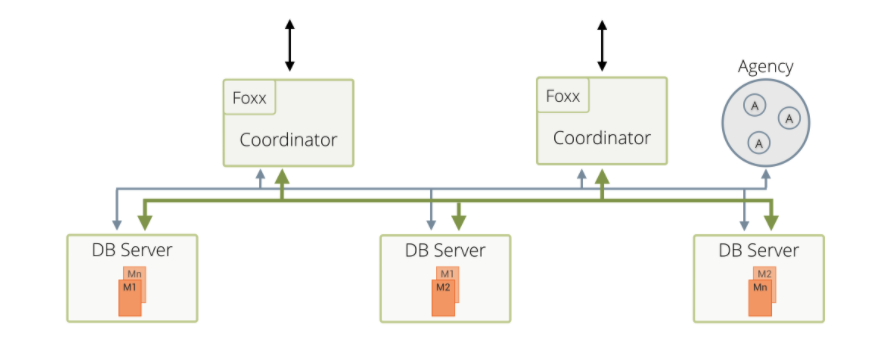
\includegraphics[width=1\textwidth]{./images/cluster-arch.png}
 	\caption{ArangoDB Cluster Architektur \cite{ADB_clusterarch}}
  \label{fig:ClusterArch}
\end{figure}


\subsubsection{Programmierschnittstellen}
ArangoDB bietet eine Vielzahl an Zugriffsmöglichkeiten.

Eine Option sind Treiber für verschiedene Programmiersprachen wie Java, NodeJS, PHP und viele andere. Des Weiteren gibt es Treiber, die von der ArangoDB Community zur Verfügung gestellt werden. \cite{ADB_driver} Diese Führen dann mit \ac{AQL} Datenabfragen auf das Cluster. 

Eine weitere Möglichkeit ist das mitgelieferte \ac{CLI}-Tool 'arangosh'. Ein einfaches Tool, welches bei Installation mitgeliefert wird, um schnelle Testabfragen an das Datenbanksystem zu stellen, jedoch ungeeignet für Produktivsysteme. \cite{ADB_arangosh}

Als letzte Zugriffsmöglichkeit bietet ArangoDB ein \ac{API}. Damit können zum Beispiel Collections, Datenbanken und Kanten über \ac{HTTP} abgefragt werden. \cite{ADB_api} Diese \ac{API} ist erweiterbar um sogennante Foxx-Microservices. Die Microservices werden in das Datenbanksystem mittels Javascript deployed. Foxx-Microservices dienen dem Nutzer der Datenbank, komplexere Berechnungen oder Abfragen datenbanknahe und optimiert auszuführen. \cite{ADB_foxx}

\subsection{Datenbankentwicklung}
\subsubsection{Systeminstallation}
Um die ArangoDB auf einen Linux Server zu installieren folgt man den Anweisungen auf der Webseite von ArangoDB.

Als ersten Schritt muss ein Repository-Schlüssel dem Paket-Manager \texttt{apt} hinzugefügt werden.
\begin{lstlisting}[language=bash]
curl -OL https://download.arangodb.com/arangodb37/DEBIAN/Release.key
sudo apt-key add - < Release.key
\end{lstlisting}
Anschließend kann über den Paketmanager die Installation folgen:
\begin{lstlisting}[language=bash]
echo 
	'deb https://download.arangodb.com/arangodb37/DEBIAN/ /' | 
	sudo tee /etc/apt/sources.list.d/arangodb.list
sudo apt-get install apt-transport-https
sudo apt-get update
sudo apt-get install arangodb3=3.7.3-1
\end{lstlisting}
Nachdem die Installation abgeschlossen wurde, kann der automatisch gestartete ArangoDB-Services wieder gestoppt werden. Diese Schritte werden nacheinander auf allen vier Nodes im Cluster ausgeführt. \cite{ADB_install}

Um nun einen ArangoDB-Cluster zu starten, haben wir den ArangoDB Starter verwendet. Der Starter ist ein \ac{CLI}-Tool, welches über Parameter die Optionen eines Datenbankservers konfiguriert. 
Für unseren Cluster haben wir für den Hauptserver (Node-4) folgende Konfiguration gewählt:
\begin{lstlisting}[language=bash]
sudo arangodb \
--starter.data-dir=/data/team38 \
--server.storage-engine=rocksdb
\end{lstlisting}
Alle weiteren Nodes wurden mit diesem Befehl mit dem Datenbankserver von Node-4 verbunden:
\begin{lstlisting}[language=bash]
sudo arangodb \
--starter.join c017-node4 \
--starter.data-dir=/data/team38 \
--server.storage-engine=rocksdb
\end{lstlisting}
\citep{ADB_starter}


\subsubsection{Datenmodellierung und Beispielschema}
Um den Use Case für den Graphen so verständlich wie möglich zu gestalten, haben wir uns ein einfaches Schema entschieden. Es besteht aus genau zwei Entitäten. Eine Collection, welche Autodaten enthält und eine weitere Collection, die die Kanten für unseren Graphen enthält. Diese Kanten zeigen von einer Auto-Entität auf eine andere Auto-Entität.
\begin{figure}[htbp] 
  	\centering
     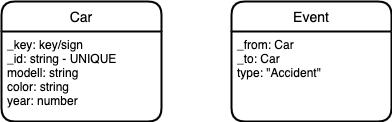
\includegraphics[width=.7\textwidth]{./images/Schema.png}
 	\caption{Implementiertes Beispielschema}
  \label{fig:DataSchema}
\end{figure}
\subsubsection{Import der Beispieldaten}
Über das Webinterface der Datenbank lassen sich für jede Collection über ein \ac{JSON}-Import Daten importieren.
Ausschnitt von Car Beispieldaten:
\lstinputlisting[linerange={1-9}]{./json/cars.json}
Ausschnitt von Event Bespieldaten:
\lstinputlisting[linerange={1-9}]{./json/events.json}
\subsubsection{AdHoc-Anfragen}

\begin{figure}[htbp] 
  	\centering
     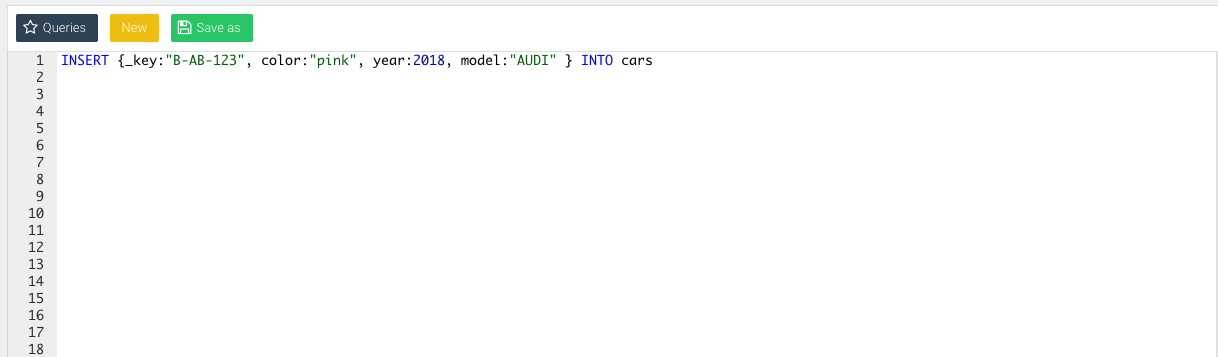
\includegraphics[width=0.9\textwidth]{./images/create.png}
 	\caption{CREATE von Dokument im Schema}
  \label{fig:DataSchema}
\end{figure}
\begin{figure}[htbp] 
  	\centering
     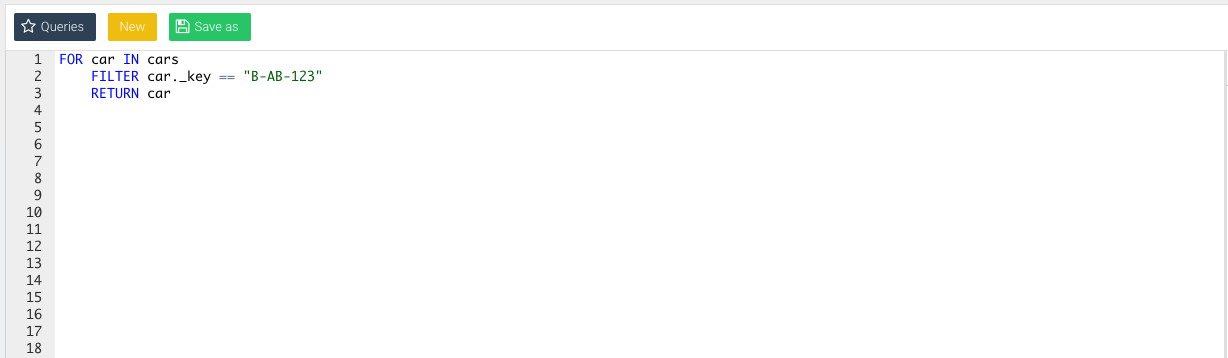
\includegraphics[width=0.9\textwidth]{./images/select.png}
 	\caption{SELECT vom erstellten Dokument}
  \label{fig:DataSchema}
\end{figure}
\begin{figure}[htbp] 
  	\centering
     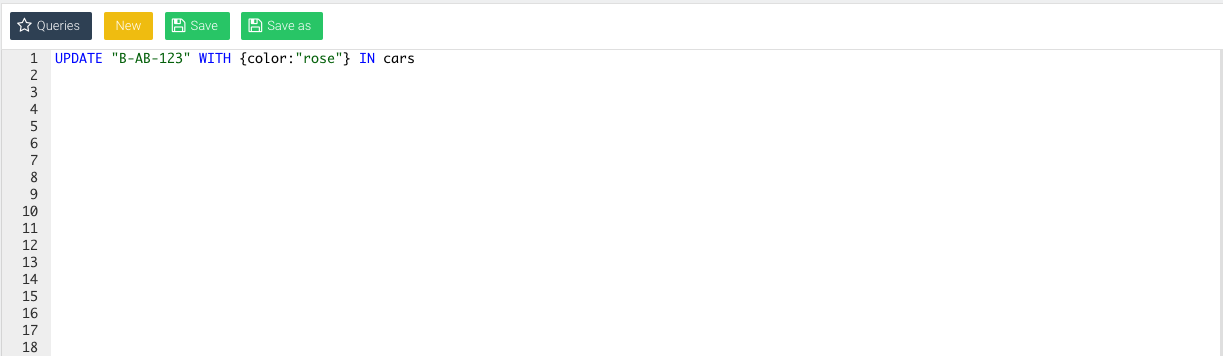
\includegraphics[width=0.9\textwidth]{./images/update.png}
 	\caption{UPDATE vom erstellten Dokument}
  \label{fig:DataSchema}
\end{figure}
\begin{figure}[htbp] 
  	\centering
     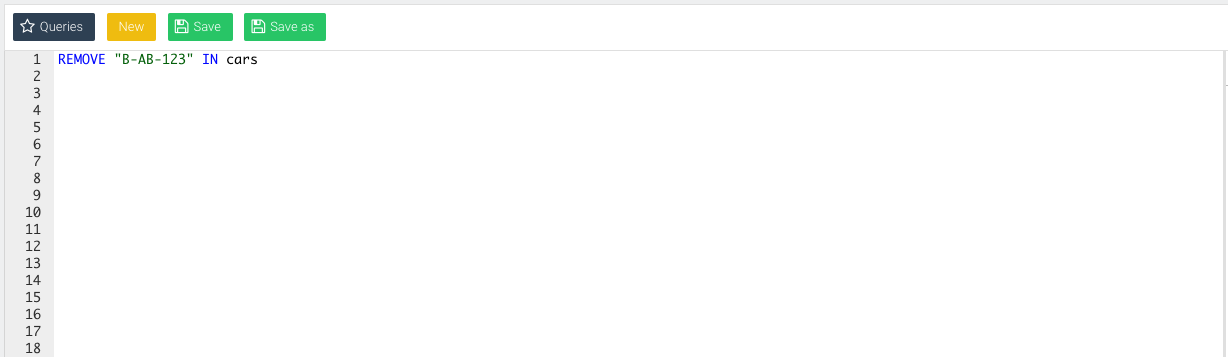
\includegraphics[width=0.9\textwidth]{./images/delete.png}
 	\caption{DELETE vom erstellten Dokument}
  \label{fig:DataSchema}
\end{figure}